\chapter{Numerical integration}
\label{cha:quadrature}

\minitoc

\section*{Introduction}
Integrals are ubiquitous in science and mathematics.
In this chapter,
we are concerned with the problem of calculating numerically integrals of the form
\begin{equation}
    \label{eq:integral}
    I = \int_{\Omega} u(\vect x) \, \d \vect x,
\end{equation}
Perhaps somewhat surprisingly,
the numerical calculation of such integrals when $n \gg 1$ is still a very active area of research today.
In this chapter,
we will focus for simplicity on the one-dimensional setting where $\Omega = [a, b] \subset \real$.
We assume throughout this chapter that the function~$u$ is Riemann-integrable.
Then, by definition,
\[
    I = \lim_{h \to 0}
    \sum_{i=0}^{n-1} u(t_i) (z_{i+1} - z_i),
\]
where $a = z_0 < \dotsb < z_n = b$ is a partition of the interval~$[a, b]$ such that the maximum spacing between successive~$x$ values is equal to~$h$,
and with $t_i \in [x_i, x_{i+1}]$ for all $i \in \{0, \dotsc, n-1\}$.

All the numerical integration formulas that we present in this chapter are based on a deterministic approximation of the form
\begin{equation}
    \label{eq:deterministic_integration}
    \widehat I = \sum_{i=0}^{n} w_i u(x_i),
\end{equation}
where~$x_0 < \dotsc < x_n$ are the \emph{integration nodes} and $w_0, \dotsc, w_n$ are the \emph{integration weights}.
In many cases, integration formulas contain a small parameter that can be changed to improve the accuracy of the approximation.
In methods based on equidistant interpolation nodes,
for example, this parameter encodes the distance between nodes and is typically denoted by~$h$,
and we often use the notation~$\widehat I_h$ to emphasize the dependence of the approximation on~$h$.
The difference~$E_h = I - \widehat I_h$ is called the \emph{integration error} or \emph{discretization error}.
The \emph{degree of precision},
defined hereafter,
is an important measure of the quality of an integration rule.
\begin{definition}
        The \emph{degree of precision} of an integration method is the smallest integer number~$d$ such that
        the integration error is zero for all $u \in \poly(d)$,
        i.e. for all the polynomials of degree less than or equal to~$d$.
\end{definition}

We observe that,
without loss of generality,
we can consider that the integration interval is equal to~$[-1, 1]$.
Indeed, using the change of variable
\begin{align}
    \notag
    \zeta\colon &[-1, 1] \to [a, b]; \\
    \label{eq:change_of_variable_integration}
                &y \mapsto \frac{b+a}{2} + \frac{(b-a)}{2} y,
\end{align}
we have
\begin{equation}
    \label{eq:change_of_variable_equivalence}
    \int_{a}^{b} u(x) \, \d x
    = \int_{-1}^{1} u\bigl(\zeta(y)\bigr) \, \zeta'(y) \, \d y
    = \frac{b-a}{2}\int_{-1}^{1} u \circ \zeta (y) \, \d y,
\end{equation}
and the right-hand side is the integral of $u \circ \zeta$ over the interval~$[-1, 1]$.

\section{The Newton--Cotes method}
\label{sec:newton_cotes}

Given a set of equidistant points $-1 = x_0 < \dotsb < x_n = 1$,
a natural method for approximating the integral~\eqref{eq:integral} of a function~$u\colon [-1, 1] \to \real$
is to first construct the interpolating polynomial~$\widehat u$ at the nodes,
and then calculate the exact integral of this polynomial.
By construction, this method is exact for polynomials of degree up to~$n$,
and so the degree of precision is equal to \emph{at least}~$n$.
Let $\varphi_0, \dotsc, \varphi_n$ denote the Lagrange polynomials associated with the integration nodes.
Then we have
\[
    I \approx \int_{-1}^{1} \widehat u(x) \, \d x
    = \int_{-1}^{1} \sum_{i=0}^{n} u(x_i) \varphi_i u(x) \, \d x
    = \sum_{i=0}^{n} u(x_i) \underbrace{\int_{-1}^{1}  \varphi_i u(x)  \, \d x}_{w_i}.
\]
The weights are independent of the function~$u$,
and so they can be calculated a priori.
The class of integration methods obtained using this approach are known as \emph{Newton--Cotes methods}.
We present a few particular cases:
\begin{itemize}
    \item
        $n = 1$, $d = 1$ (trapezoidal rule):
        \begin{equation}
            \label{eq:trapezoidal_rule}
            \int_{-1}^{1} u(x) \, dx
            \approx u(-1) + u(1).
        \end{equation}

    \item
        $n = 2$, $d = 3$ (Simpson's rule):
        \begin{equation}
            \label{eq:simpsons}
            \int_{-1}^{1} u(x) \, dx
            \approx \frac{1}{3} u(-1) + \frac{4}{3} u(0) + \frac{1}{3} u(1).
        \end{equation}

    \item
        $n = 3$, $d = 3$ (Simpson's $\frac{3}{8}$ rule):
        \[
            \int_{-1}^{1} u(x) \, dx
            \approx \frac{1}{4} u(-1) + \frac{3}{4} u(-1/3) + \frac{3}{4} u(1/3) + \frac{1}{4} u(1).
        \]

    \item
        $n = 4$, $d = 5$ (Bode's rule):
        \[
            \int_{-1}^{1} u(x) \, dx
            \approx \frac{7}{45} u(-1) + \frac{32}{45} u\left(-\frac{1}{2}\right) + \frac{12}{45} u\left(0\right) + \frac{32}{45} u\left(\frac{1}{2}\right) + \frac{7}{45} u(1).
        \]
\end{itemize}
In principle,
this approach could be employed in order to construct integration rules of arbitrary high degree of precision.
In practice, however, the weights become more and more imbalanced as the number of interpolation points increases,
with some of them becoming negative.
As a result, roundoff errors become increasingly detrimental to accuracy.
In addition, in cases where the interpolating polynomial does not converge to~$u$,
for example if~$u$ is Runge's function,
the approximate integral may not converge to the correct value in the limit as~$n \to \infty$,
even in exact arithmetic!

\begin{remark}
    Note that,
    although it is based on a quadratic polynomial interpolation,
    Simpson's rule~\eqref{eq:simpsons} has a degree of precision equal to~$3$.
    This is because any integration rule with nodes and weights symmetric around $x=0$ is exact for odd functions,
    in particular $x^3$.
    Likewise, the degree of precision of Bode's rule is equal to 5.
\end{remark}

\section{Composite methods with equidistant nodes}
\label{sec:composite_methods}
A natural alternative to the approach presented in~\cref{sec:newton_cotes}
is to construct an integration rule using piecewise polynomial interpolation,
which we studied in~\cref{sub:piecewise_interpolation}.
After partitioning the integration interval in a number of subintervals,
the integral can be approximated by using one of the rules presented in~\eqref{sec:newton_cotes} within each subinterval.

\paragraph{Composite trapezoidal rule.}
Let us illustrate the composite approach with an example.
To this end,
we introduce a partition $a = x_0 < \dotsb < x_n = b$ of the interval $[a, b]$ and
assume that the nodes are equidistant with $x_{i+1} - x_i = h$.
Using~\eqref{eq:change_of_variable_equivalence},
we first generalize~\eqref{eq:trapezoidal_rule} to an interval~$[x_i, x_{i+1}]$ as follows:
\[
    \int_{x_i}^{x_{i+1}} u(x) \, \d x
    = \int_{-1}^{1} u \circ \zeta (y) \, \d y
    \approx u \circ \zeta(-1)  + u \circ \zeta(1)
    = \frac{h}{2} \bigl(u(x_i) + u(x_{i+1})\bigr),
\]
where $\approx$ in this equation indicates approximation using the trapezoidal rule.
Applying this approximation to each subinterval of the partition,
we obtain the composite trapezoidal rule:
\begin{align}
    \notag
    \int_{a}^{b} u(x) \, \d x
    &= \sum_{i=0}^{n-1} \int_{x_i}^{x_{i+1}} u(x) \, \d x
    \approx
    \frac{h}{2}\sum_{i=0}^{n-1} \bigl( u(x_i) + u(x_{i+1}) \bigr) \\
    \label{eq:composite_trapezoidal_rule}
    &= \frac{h}{2} \bigl( u(x_0) + 2 u(x_1) + 2 u(x_2) + \dotsb + 2 u(x_{n-2}) + 2 u(x_{n-1}) + u(x_n) \bigr).
\end{align}
Like the trapezoidal rule~\eqref{eq:trapezoidal_rule},
the composite trapezoidal rule~\eqref{eq:composite_trapezoidal_rule} has a degree of precision equal to 1.
However,
the integration error of the method depends on the parameter~$h$,
which represents the width of each subinterval:
for very small~$h$,
equation~\eqref{eq:composite_trapezoidal_rule} is expected to provide a good approximation of the integral.
An error estimate can be obtained directly from the formula in~\cref{theorem:interpolation_error} for the interpolation error,
provided that we assume that~$u \in C^2([a, b])$.

\begin{theorem}
    [Integration error for the composite trapezoidal rule]
    Let $\widehat I_h$ denote the approximate integral calculated using~\eqref{eq:composite_trapezoidal_rule}.
    Then
    \begin{equation}
        \label{eq:error_bound_trapezoidal}
        \bigl\lvert I - \widehat I_h \bigr\rvert
        \leq \frac{b-a}{12} C_2 h^2,
        \qquad
        C_2 := \sup_{\xi \in [a, b]} \abs*{u''(\xi)}.
    \end{equation}
\end{theorem}

\begin{proof}
Denoting by~$\widehat u_h$ the piecewise linear interpolation of~$u$,
we have
\[
    \int_{x_{i}}^{x_{i+1}} u(x) - \widehat u(x) \, \d x
    = \frac{1}{2} \int_{x_{i}}^{x_{i+1}} u''\bigl(\xi(x)\bigr) (x - x_{i}) (x - x_{i+1}) \, \d x.
\]
Since $(x - x_i) (x - x_{i+1})$ is nonpositive over the interval $[x_i, x_{i+1}]$,
we deduce that
\[
    \abs*{\int_{x_{i}}^{x_{i+1}} u(x) - \widehat u(x) \, \d x}
    \leq \left( \sup_{\xi \in [a, b]} \abs*{u''(\xi)} \right) \int_{x_{i}}^{x_{i+1}} (x - x_{i}) (x_{i+1} - x) \, \d x
    = C_2 \frac{h^3}{12}.
\]
Summing the contributions of all the intervals,
we obtain
\[
    \bigl\lvert I - \widehat I_h \bigr\rvert
    \leq \sum_{i=0}^{n-1} \abs*{\int_{x_i}^{x_{i+1}} u(x) - \widehat u(x) \, \d x }
    \leq n \times C_2 \frac{h^3}{12} = \frac{b-a}{12} C_2 h^2,
\]
which concludes the proof.
\end{proof}

The integration error therefore scales as~$\mathcal O(h^2)$.
(Strictly speaking, we have shown only that the integration error admits an upper bound that scales at $\mathcal O(h^2)$,
but it turns out that the dependence on~$h$ of this bound is optimal).

\paragraph{Composite Simpson rule.}
The composite Simpson rule is derived in~\cref{exercise:composite_simpson}.
Given an odd number $n+1$ of equidistant points $a = x_0 < x_1 < \dotsb < x_n = b$,
this rule is given by
\begin{equation}
    \label{eq:composite_simpson}
    \widehat I_h = \frac{h}{3} \Bigl( u(x_0) + 4 u(x_1) + 2 u(x_2) + 4 u(x_3) + 2 u_(x_4) + \dotsb + 2 u(x_{n-2}) + 4 u(x_{n-1}) + u(x_n)\Bigr).
\end{equation}
This approximation is obtained by integrating the piecewise quadratic interpolant
over a partition of the integration interval into $n/2$ subintervals of equal width.
Obtaining an optimal error estimate,
in terms of the dependence on~$h$,
for this integration formula is slightly more involved.

\begin{theorem}
    [Integration for the composite Simpson rule]
    Let $\widehat I_h$ denote the approximate integral calculated using~\eqref{eq:composite_simpson}.
    Then
    \begin{equation}
        \label{eq:error_bound_simpson}
        \bigl\lvert I - \widehat I_h \bigr\rvert
        \leq (b-a)\frac{C_4 h^4}{180},
        \qquad
        C_4 := \sup_{\xi \in [a, b]} \abs*{u^{(4)}(\xi)}.
    \end{equation}
\end{theorem}
\begin{proof}
For a given subinterval~$[x_{2i}, x_{2i+2}]$,
let us denote by~$\widehat u_2$ the quadratic interpolating polynomial at $x_{2i}, x_{2i+1}, x_{2i+2}$,
and by $\widehat u_3(\placeholder; \alpha)$ the cubic interpolating polynomial relative to the nodes $x_{2i}, x_{2i+1}, x_{2i+2}, \alpha$,
for some $\alpha \in [x_{2i}, x_{2i+1}]$ that does not coincide with the integration nodes.
We have
\begin{align}
    \label{eq:composite_simpson_error}
    \int_{x_{2i}}^{x_{2i+2}} u(x) - \widehat u_2(x) \, \d x
    &= \int_{x_{2i}}^{x_{2i+2}} u(x) - \widehat u_3(x; \alpha)  \, \d x + \int_{x_{2i}}^{x_{2i+2}} \widehat u_3(x; \alpha) - \widehat u_2(x)  \, \d x.
\end{align}
The second term on the right-hand side is zero,
because the integrand is a cubic polynomial with zeros at $x_{2i}$, $x_{2i+1}$ and $x_{2i+2}$,
and because
\[
    \int_{x_{2i}}^{x_{2i+2}} (x - x_{2i}) (x - x_{2i+1}) (x - x_{2i+2}) = 0.
\]
% (The integral is zero because the integrand is odd around the vertical axis $x = x_{2i+1}$.)
By~\cref{theorem:interpolation_error},
the first term in~\eqref{eq:composite_simpson_error} is bounded from above as follows:
\begin{align*}
    \abs*{\int_{x_{2i}}^{x_{2i+2}} u(x) - \widehat u_3(x; \alpha)  \, \d x}
    &\leq \int_{x_{2i}}^{x_{2i+2}} \left\lvert \frac{u^{(4)} \bigl(\xi(x)\bigr)}{24} (x-x_{2i})(x- x_{2i+1}) (x-x_{2i+2}) (x - \alpha) \right\rvert \, \d x \\
    &\leq \frac{C_4}{24} \int_{x_{2i}}^{x_{2i+2}} \bigl\lvert (x-x_{2i})(x- x_{2i+1}) (x-x_{2i+2}) (x - \alpha) \bigr\rvert \, \d x.
\end{align*}
This inequality is valid for any $\alpha \in A := [x_{2i}, x_{2i+2}] \backslash \{x_{2i}, x_{2i+1}, x_{2i+2}\}$.
Denoting by $h(\alpha)$ the integral on the right-hand side,
we observe that
\[
    \lim_{\alpha \to x_{2i+1}} h(\alpha) =
    \int_{x_{2i}}^{x_{2i+2}} (x-x_{2i})(x- x_{2i+1})^2 (x_{2i+2} - x) \, \d x = \frac{4}{15} h^5.
\]
Therefore, we conclude that
\[
    \abs*{\int_{x_{2i}}^{x_{2i+2}} u(x) - \widehat u_2(x)  \, \d x}
    \leq \inf_{\alpha \in A} \abs*{\int_{x_{2i}}^{x_{2i+2}} u(x) - \widehat u_3(x; \alpha)  \, \d x} \leq \frac{C_4}{90} h^5.
\]
Summing the contributions of all the subintervals,
we finally obtain
\begin{equation}
    \label{eq:scaling_error}
    \abs{I - \widehat I_h} \leq  \frac{n}{2} \times \frac{C_4 h^5}{90} = (b-a)\frac{C_4 h^4}{180},
\end{equation}
which concludes the proof.
\end{proof}

\begin{remark}
The cancellation of the second term in~\eqref{eq:composite_simpson_error} also follows from the fact that
the degree of precision of the Simpson rule~\eqref{eq:simpsons} is equal to~3,
and so
\[
    \int_{x_{2i}}^{x_{2i+2}} \widehat u_3(x) - \widehat u_2(x)  \, \d x = \frac{1}{3} (\widehat u_3 - \widehat u_2)(x_{2i}) + \frac{4}{3} (\widehat u_3 - \widehat u_2)(x_{2i+1}) + \frac{1}{3} (\widehat u_3 - \widehat u_2)(x_{2i+2}) = 0,
\]
where we used the short-hand notation $\widehat u_3(x) = \widehat u_3(x; \alpha)$.
\end{remark}

\paragraph{Estimating the error a posteriori.}
In practice,
it is useful to be able to estimate the integration error so that,
if the error is deemed too large,
a better approximation of the integral can be calculated by using a smaller value for the step size~$h$.
Calculating the exact error $I - \widehat I_h$ is impossible in general,
because this would require to know the exact value of the integral,
but it is possible to calculate a rough approximation of the error based on two numerical approximations of the integral,
as we illustrate formally hereafter for the composite Simpson rule.

Suppose that $\widehat I_{2h}$ and $\widehat I_{h}$ are two approximations of the integral,
calculated using the composite Simpson rule with step size $2h$ and $h$, respectively.
If we assume that the error proportionally to~$\mathcal O(h^4)$ as~\eqref{eq:scaling_error} suggests,
then it holds approximately that
\begin{equation}
    \label{eq:relation_errors}
    I - \widehat I_{h} \approx \frac{1}{2^4} (I - \widehat I_{2h}).
\end{equation}
This implies that
\[
    I - \widehat I_{2h} = (I - \widehat I_h) + (I_h - \widehat I_{2h}) \approx \frac{1}{16}(I - \widehat I_{2h}) + (\widehat I_h - \widehat I_{2h}).
\]
Rearranging this equation gives an approximation of the error for $\widehat I_{2h}$:
\[
    I - \widehat I_{2h} \approx \frac{16}{15} (\widehat I_h - \widehat I_{2h}).
\]
Using~\eqref{eq:relation_errors},
we can then derive an error estimate for $\widehat I_h$:
\begin{equation}
    \label{eq:integration_error_approximation}
    \abs{I - \widehat I_{h}} \approx \frac{1}{15} \abs{\widehat I_h - \widehat I_{2h}}.
\end{equation}
The right-hand side can be calculated numerically,
because it does not depend on the exact value of the integral.
In practice,
the two sides of~\eqref{eq:integration_error_approximation} are often very close for small~$h$.
In the code example below,
we approximate the integral
\begin{equation}
    \label{eq:integral_example}
    I = \int_{0}^{\frac{\pi}{2}} \cos(x) \, \d x = 1
\end{equation}
for different step sizes
and compare the exact error with the approximate error obtained using~\eqref{eq:integration_error_approximation}.
The results obtained are summarized in~\cref{tab:discretization_error},
which shows a good match between the two quantities.
\begin{table}[ht!]
    \def\arraystretch{1.5}
    \centering
    \caption{Comparison between the exact integration error and the approximate integration error calculated using~\eqref{eq:integration_error_approximation}.}
    \label{tab:discretization_error}
    \begin{tabular}{|c|c|c|}
        \hline
        $h$ & Exact error $\abs{I - \widehat I_h}$ & Approximate error $\frac{1}{15}\abs{\widehat I_h - \widehat I_{2h}}$
        \\ \hline
        $2^{-4}$ & $5.166847063531321 \times 10^{-7}$ & $5.185892840930961 \times 10^{-7}$
        \\ \hline
            $2^{-5}$ & $3.226500089326123 \times 10^{-8}$ & $3.229464703065806 \times 10^{-8}$
        \\ \hline
                $2^{-6}$ & $2.0161285974040766 \times 10^{-9}$ & $2.016591486390477 \times 10^{-9}$
        \\ \hline
                    $2^{-7}$ & $1.2600120946615334 \times 10^{-10}$ & $1.260084925291949 \times 10^{-10}$
        \\ \hline
    \end{tabular}
\end{table}

\begin{minted}[fontsize=\footnotesize]{julia}
# Composite Simpson's rule
function composite_simpson(u, a, b, n)
    # Integration nodes
    x = LinRange(a, b, n + 1)
    # Evaluation of u at the nodes
    ux = u.(x)
    # Step size
    h = x[2] - x[1]
    # Approximation of the integral
    return (h/3) * sum([ux[1]; ux[end]; 4ux[2:2:end-1]; 2ux[3:2:end-2]])
end
# Function to integrate
u(x) = cos(x)
# Integration bounds
a, b = 0, π/2
# Exact integral
I = 1.0
# Number of subintervals
ns = [8; 16; 32; 64; 128]
# Approximate integrals
Î = composite_simpson.(u, a, b, ns)
# Calculate exact and approximate errors
for i in 2:length(ns)
    println("Exact error: $(I - Î[i]), ",
            "Approx error: $((Î[i] - Î[i-1])/15)")
end
\end{minted}

\section{Richardson extrapolation and Romberg's method}
In the previous section,
we showed how the integration error could be approximated based on two approximations of the integral with different step sizes.
The aim of this section is to show that,
by cleverly combining two approximations $\widehat I_h$ and $\widehat I_{2h}$ of an integral,
an approximation even better than $\widehat I_h$ can be constructed.

This approach is based on \emph{Richardson's extrapolation},
which is a general method for accelerating the convergence of sequences,
with applications beyond numerical integration.
The idea is the following:
assume that $J(h)$ is an approximation with step size~$h$ of some unknown quantity~$J_* = \lim_{h\to 0} J(h)$,
and that we have access to evaluations of $J$ at $h, h/2, h/4, h/8 \dotsc$.
If $J$ extends to a smooth function over $[0, H]$,
then by Taylor expansion it holds that
\[
    J(\eta) = J(0) + J'(0) \eta + J''(0) \frac{\eta^2}{2} + J^{(3)}(0) \frac{\eta^3}{3!} + \dotsb + J^{(k)}(0) \frac{\eta^k}{k!} + \mathcal O(\eta^{k+1}).
\]

\paragraph{Elimination of the linear error term.}
Let us assume that $J'(0) \neq 0$,
so that the leading order term after the constant $J(0)$ scales as~$\eta$.
Then we have
\begin{align*}
    J(h) &= J(0) + J'(0) h + \mathcal O(h^2) \\
    J(h/2) &= J(0) + J'(0) \frac{h}{2} + \mathcal O(h^2).
\end{align*}
We now ask the following question:
can we combine linearly $J(h)$ and $J(h/2)$ in order to construct an approximation $J_1(h/2)$ of~$J(0)$ with an error scaling as $\mathcal O(h^2)$?
Employing the ansatz
\(
    J_1(h/2) = \alpha J(h) + \beta J(h/2),
\)
we calculate
\begin{equation}
    \label{eq:expansion_richardson}
    J_1(h/2) = (\alpha + \beta) J(0) + J'(0) h \left(\alpha + \frac{1 - \alpha}{2}\right) + \mathcal O(h^2).
\end{equation}
Since we want this expression to approximate $J(0)$ for small~$h$,
we need to impose that $\alpha + \beta = 1$.
Then, in order for the term multiplying~$h$ to cancel out,
we require that
\[
    \alpha + \frac{1 - \alpha}{2} = 0
    \qquad \Leftrightarrow \qquad
    \alpha = - 1.
\]
This yields the formula
\begin{equation}
    \label{eq:richardson}
    J_1(h/2) = 2J(h/2) - J(h).
\end{equation}
Notice that, in the case where $J$ is a linear function,
$J_1(h/2)$ is exactly equal to~$J(0)$.
This reveals a geometric interpretation of~\eqref{eq:richardson}:
the approximation $J_1(h/2)$ is simply the $y$ intercept of the straight line passing through the points $\bigl(h/2, J(h/2)\bigr)$ and $\bigl(h, J(h)\bigr)$.

\paragraph{Elimination of the quadratic error term.}
If we had tracked the coefficient of $h^2$ in the previous paragraph,
we would have obtained instead of~\eqref{eq:expansion_richardson} the following equation:
\[
    J_1(h/2) = J(0) - J^{(3)}(0) \frac{h^2}{4} + \mathcal O(h^3).
\]
Provided that we have access also to $J(h/4)$,
we can also calculate
\[
   J_1(h/4) = 2J(h/4) - J(h/2) = J(0) - J^{(3)}(0) \frac{h^2}{16} + \mathcal O(h^3).
\]
At this point,
it is natural to wonder whether we can combine $J_1(h/2)$ and $J_1(h/4)$ in order to produce an even better approximation of $J(0)$.
Applying the same reasoning as in the previous section leads us to introduce
\[
    J_2(h/4) = \frac{4 J_1(h/2) - J_2(h/4)}{4 - 1} = J(0) + \mathcal O(h^3).
\]
This is an exact approximation of $J(0)$ if $J$ is a quadratic polynomial,
indicating that $J_2(h/4)$ is simply the $y$ intercept of the quadratic polynomial interpolating the function~$J$ through the three points
$\bigl(h/4, J(h/4)\bigr)$, $\bigl(h/2, J(h/2)\bigr)$ and $\bigl(h, J(h)\bigr)$.

\paragraph{Elimination of higher order terms.}
The procedure above can be repeated in order to eliminate terms of higher and higher orders.
The following schematic illustrates,
for example, the calculation of an approximation $J_3(h/8) = J(0) + \mathcal O(h^4)$.
\[
    \begin{tikzcd}[cramped, sep=small]
        J(h) \arrow[dr]  \\
        J(h/2) \arrow[r] \arrow[dr] & J_1(h/2) \arrow[dr]  \\
        J(h/4) \arrow[r] \arrow[dr] & J_1(h/4) \arrow[r] \arrow[dr] & J_2(h/4) \arrow[dr]  \\
        J(h/8) \arrow[r] & J_1(h/8) \arrow[r] & J_2(h/8) \arrow[r] & J_3(h/8) \\
        \mathcal O(h) & \mathcal O(h^2) & \mathcal O(h^3) & \mathcal O(h^4).
    \end{tikzcd}
\]
Here, the last row indicates the scaling of the error with respect to the parameter $h$ in the limit as~$h \to 0$.
The linear combination in order to calculate $J_{i} (h/2^i)$ is always of the form
\[
    J_i(h/2^i) = \frac{2^i J_{i-1} (h/2^i) - J_{i-1}(h/2^{i-1})}{2^i - 1}, \qquad J_0 = J.
\]
In practice we calculate the values taken by $J, J_1, J_2, \dotsc$ at specific values of~$h$,
but these are in fact functions of~$h$.
In~\cref{fig:richardson},
we plot these functions when~$J(h) = 1 + \sin(h)$.
It appears clearly from the figure that,
for sufficiently small~$h$,
$J_3(h)$ provides the most precise approximation of $J(0) = 1$.
Constructing the functions in Julia can be achieved in just a few lines of code.
\begin{minted}[fontsize=\footnotesize]{julia}
    J(h) = 1 + sin(h)
    J_1(h) = 2J(h) - J(2h)
    J_2(h) = (4J_1(h) - J_1(2h))/3
    J_3(h) = (8J_2(h) - J_2(2h))/7
\end{minted}
\begin{figure}[ht]
    \centering
    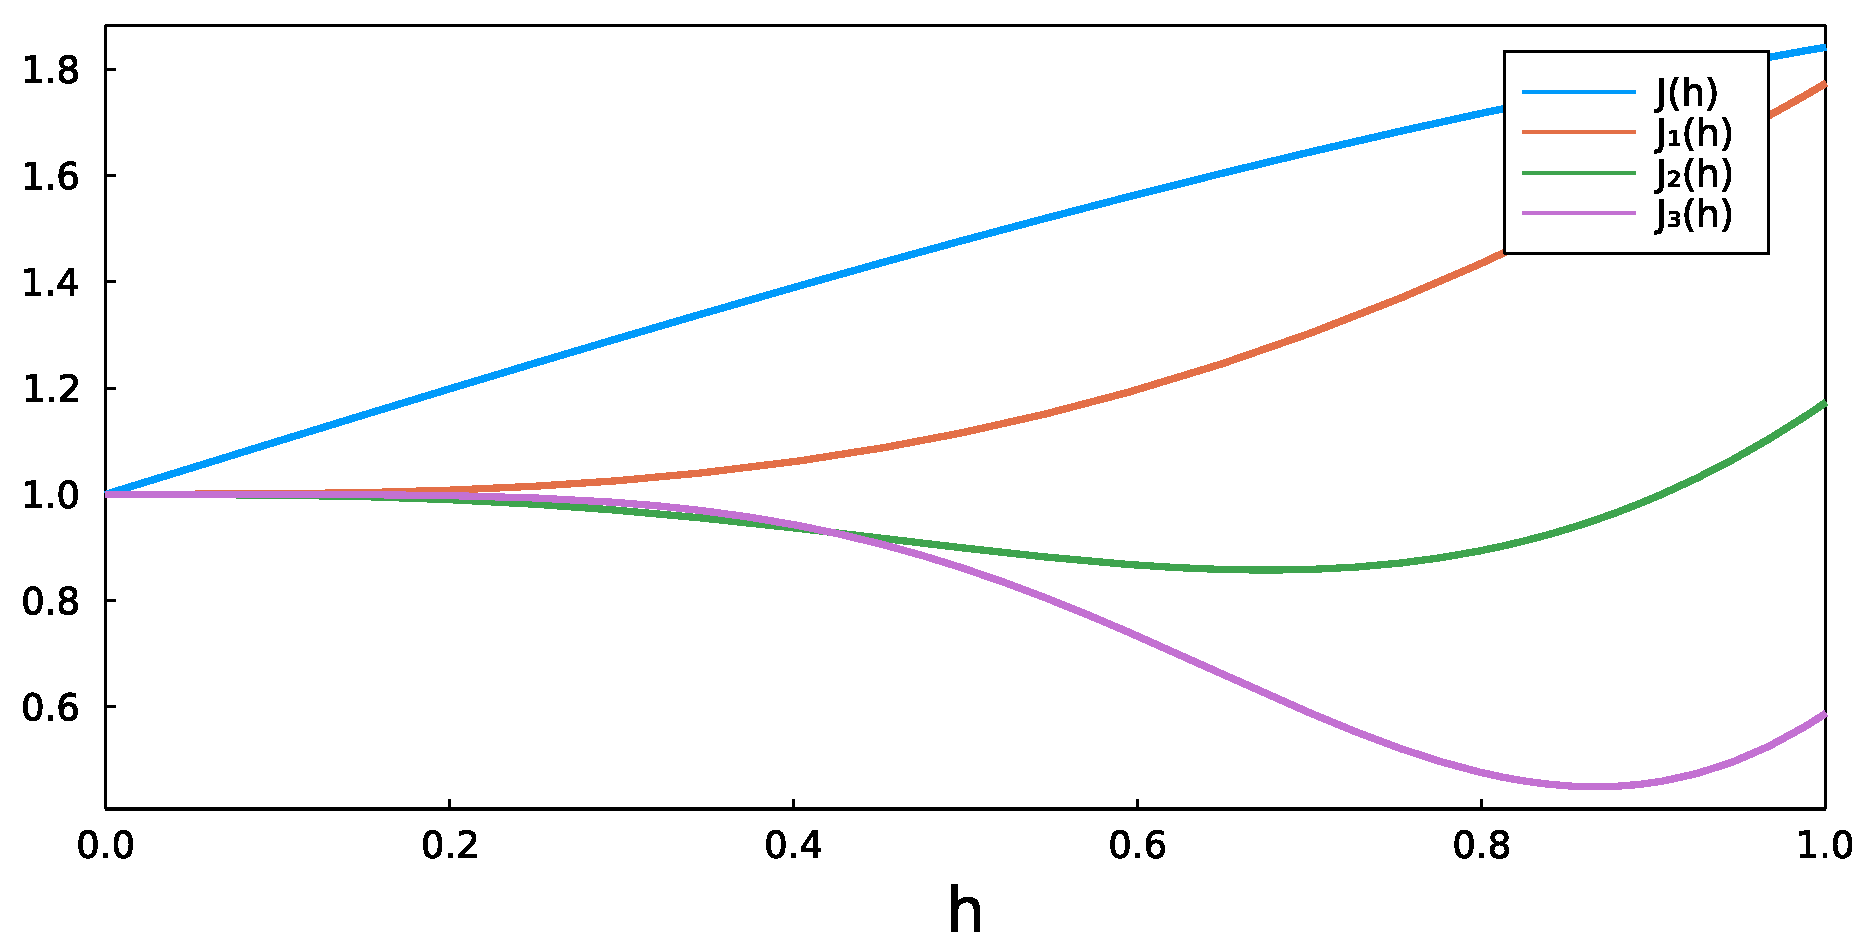
\includegraphics[width=0.8\linewidth]{figures/richardson.pdf}
    \caption{Illustration of the functions $J_1$, $J_2$ and $J_3$ constructed by Richardson extrapolation.}%
    \label{fig:richardson}
\end{figure}

\paragraph{Generalization.}
Sometimes,
it is known a priori that the Taylor development of the function~$J$ around zero contains only even powers of~$h$.
In this case, the Richardson extrapolation procedure can be slightly modified in order to produce approximations with errors scaling as~$\mathcal O(h^4)$,
then~$\mathcal O(h^6)$, then~$\mathcal O(h^8)$, etc.
This procedure is illustrated below:
\[
    \begin{tikzcd}[cramped, sep=small]
        J(h) \arrow[dr]  \\
        J(h/2) \arrow[r] \arrow[dr] & J_1(h/2) \arrow[dr]  \\
        J(h/4) \arrow[r] \arrow[dr] & J_1(h/4) \arrow[r] \arrow[dr] & J_2(h/4) \arrow[dr]  \\
        J(h/8) \arrow[r] & J_1(h/8) \arrow[r] & J_2(h/8) \arrow[r] & J_3(h/8) \\
        \mathcal O(h^2) & \mathcal O(h^4) & \mathcal O(h^6) & \mathcal O(h^8).
    \end{tikzcd}
\]
This time, the linear combinations required for populating this table are given by
\begin{equation}
    \label{eq:generalized_richardson}
    J_i(h/2^i) = \frac{2^{2i} J_{i-1} (h/2^i) - J_{i-1}(h/2^{i-1})}{2^{2i} - 1}.
\end{equation}

\paragraph{Application to integration: Romberg's method}
Romberg's integration method consists of applying Richardson's extrapolation to the function
\[
    J(h) = \widehat I_h = u(x_0) + 2 u(x_1) + 2 u(x_2) + \dotsb + 2 u(x_{n-1}) + 2 u(x_n), \qquad h \in \left\{ \frac{b-a}{n}: n \in \nat\right\}.
\]
where $a = x_0 < x_1 < \dotsb < x_n = b$ are equidistant nodes.
The right-hand side of this equation is simply the composite trapezoidal rule with step size~$h$.
It is possible to show, see for example~\cite[Property 9.3]{MR2265914},
that~$J(h)$ may be expanded as follows:
\[
    \forall k \in \nat, \qquad
    J(h) = I + \alpha_1 h^2 + \alpha_2 h^4 + \cdots + \alpha_k h^{2k} + \mathcal O(h^{2k+2}).
\]
Richardson's extrapolation~\eqref{eq:generalized_richardson} can therefore be employed in order to compute approximations of the integral with increasing accuracy.
The convergence of Romberg's method for calculating the integral~\eqref{eq:integral_example} is illustrated in~\cref{fig:romberg}.
\begin{figure}[ht]
    \centering
    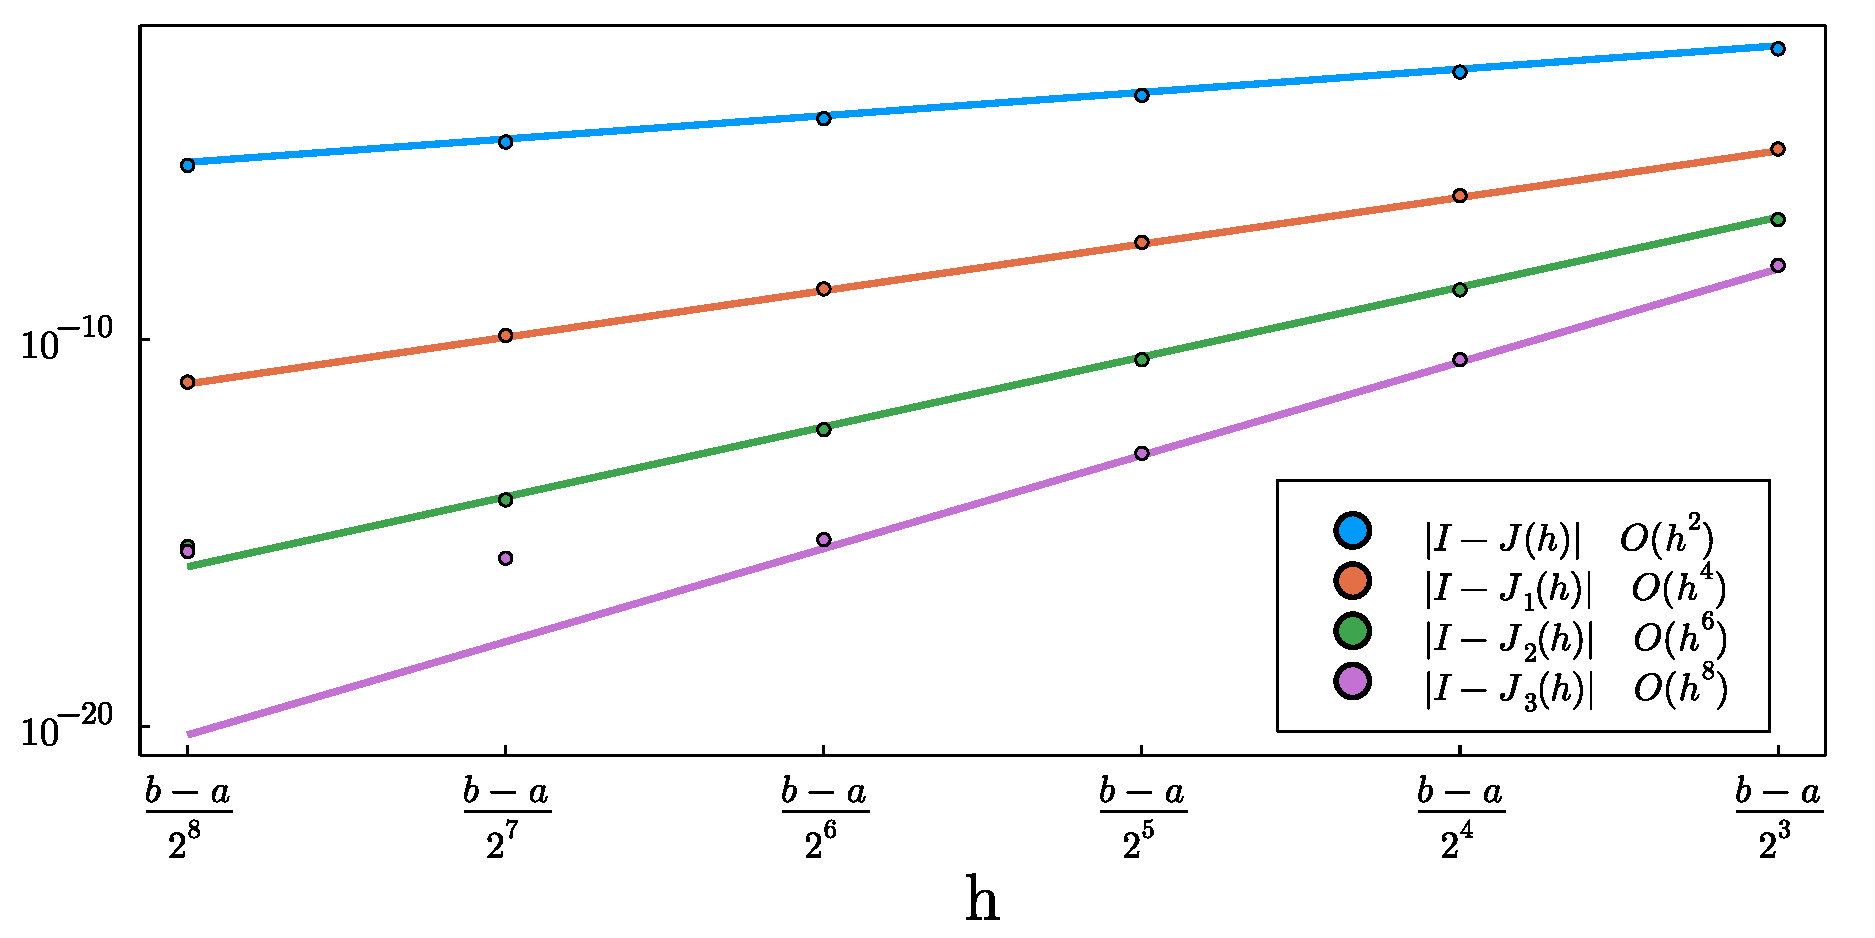
\includegraphics[width=0.95\linewidth]{figures/romberg.pdf}
    \caption{Convergence of Romberg's method. The straight lines correspond to the monomial functions $f(h) = C_i h^i$,
    with $i = 2, 4, 6, 8$ and for appropriate constants $C_i$.
    We observe a good agreement between the observed and theoretical convergence rates.}%
    \label{fig:romberg}
\end{figure}

\section{Methods with non-equidistant nodes}
The Newton--Cotes method relies on equidistant integration nodes,
and the only degrees of freedom are the integration weights.
If the nodes are not fixed,
then additional degrees of freedom are available,
and these can be leveraged in order to construct a better integration formula.
The total number of degrees of freedom for a general integration rule of the form~\eqref{eq:deterministic_integration} is $2n + 2$ which,
in principle, should enable to construct an integration rule with a degree of precision equal to~$2n+1$.

A necessary condition for an integration rule of the form~\eqref{eq:deterministic_integration} to have a degree of precision
equal to $2 n +1$ is that it integrates exactly all the monomials of degree $0$ to~$2 n+1$.
This condition is also sufficient because,
assuming that it is satisfied,
we have by linearity of the functionals~$I$ and $\widehat I$ that
\begin{align*}
    \widehat I\left(\alpha_0 + \alpha_1 x + \dotsb + \alpha_{2n+1} x^{2n+1}\right)
    &= \alpha_0 \widehat I(1) + \alpha_1 \widehat I(x) + \dotsb + \alpha_{2n+1} \widehat I\left(x^{2n+1}\right) \\
    &= \alpha_0 I(1) + \alpha_1 I(x) + \dotsb + \alpha_{2n+1} I\left(x^{2n+1}\right) \\
    &= I\left(\alpha_0 + \alpha_1 x + \dotsb + \alpha_{2n+1} x^{2n+1}\right),
\end{align*}
Here $I(u)$ and $\widehat I(u)$ denote respectively the exact integral of~$u$ and its approximate integral using~\eqref{eq:deterministic_integration}.
In order to find the nodes and weights of the integration rule,
we can therefore solve the following nonlinear system of $2n+2$ equations with $2n+2$ unknowns:
\begin{align}
    \label{eq:system_gauss_legendre}
    \sum_{i=0}^{n} w_i x_i^{d} &= \int_{-1}^{1} x^d \, \d x, \qquad d = 0, \dotsc, 2n+1.
\end{align}
The quadrature rule thus obtained is called the \emph{Gauss--Legendre quadrature}.
\begin{example}
Let us derive the Gauss--Legendre quadrature with $n + 1 = 2$ nodes.
The system of equations that we need to solve in this case is the following:
\begin{align*}
    w_0 + w_1 = 2,
    \qquad w_0 x_0 + w_1 x_1 = 0,
    \qquad w_0 x_0^2 + w_1 x_1^2 = \frac{2}{3},
    \qquad w_0 x_0^3 + w_1 x_1^3 = 0.
\end{align*}
The solution to these equations is given by
\[
    - x_0 = x_1 = \frac{\sqrt{3}}{3}, \qquad w_0 = w_1 = 1.
\]
\end{example}

\paragraph{Connection with orthogonal polynomials.}
Let $(L_n)_{n \in \nat}$ denote the Legendre polynomials,
i.e. the orthogonal polynomials with for the inner product
\[
    \ip{f, g} = \int_{-1}^{1} f(x) g(x) \, \d x.
\]
The nodes and weights of the Gauss--Legendre quadrature rules can be obtained constructively from Legendre polynomials,
as shown in~\cref{sub:orthogonal_integration}.
We shall now demonstrate this connection in much more direct manner.
Specifically, we prove that the integration nodes are given by the roots of a Legendre polynomial.
\begin{theorem}
    \label{theorem:gauss_legendre_connection_polynomials}
    For every $n \in \nat$,
    there exists a unique solution to the system of equations~\eqref{eq:system_gauss_legendre}.
    The nodes $(x_i)_{i \in \{0,\dotsc, n\}}$ are the roots of $L_{n+1}$
    and the weights are given by
    \begin{equation}
        \label{eq:weights_gauss}
        w_i = \int_{-1}^{1} \ell_i(x) \, \d x, \qquad i \in \{ 1, \dotsc, n\},
    \end{equation}
    where $\ell_i$ is the Lagrange polynomial
    \[
        \frac{(x - x_0) \dotsb (x - x_{i-1})(x- x_{i+1}) \dotsb (x - x_n)}
        {(x_i - x_0) \dotsb (x_i - x_{i-1})(x_i- x_{i+1}) \dotsb (x_i - x_n)}.
    \]
    In addition, the weights are all positive.
\end{theorem}
\begin{proof}
    We show first that the solution to~\eqref{eq:system_gauss_legendre} exists,
    then that it is unique,
    and finally that the weights are positive.
    \paragraph{Existence.}
    We begin by showing that,
    if $(x_i)_{i \in \{0,\dotsc n\}}$ are the roots of~$L_{n+1}$ and the weights are defined from~\eqref{eq:weights_gauss},
    then the equations~\eqref{eq:system_gauss_legendre} are satisfied.
    To this end,
    it is sufficient to show that for all $p \in \poly(2n + 1)$,
    \begin{equation}
        \label{eq:gauss_legendre_equation}
        \int_{-1}^{1} p(x) \, \d x = \sum_{i=0}^{n} w_i p(x_i).
    \end{equation}
    Take $p \in \poly(2n + 1)$ and let $q \in \poly(n)$ and $r \in \poly(n)$ be the polynomials such that
    \[
        p(x) = q(x) L_{n+1}(x) + r(x).
    \]
    The quotient $q$ and the remainder $r$ can be obtained by Euclidean division.
    Since $L_{n+1}$ is orthogonal to any polynomial in~$\poly(n)$,
    in particular $q$,
    and the nodes $(x_i)_{i \in \{0,\dotsc n\}}$ are the roots of~$L_{n+1}$,
    it holds that
    \begin{equation}
        \label{eq:intermediate_gauss}
        \int_{-1}^{1} p(x) \, \d x
        - \sum_{i=0}^{n} w_i p(x_i)
        = \int_{-1}^{1} r(x) \, \d x
        - \sum_{i=0}^{n} w_i r(x_i).
    \end{equation}
    Given that $r \in \poly(n)$,
    the remainder $r$ must coincides with its polynomial interpolation at the points $x_0, \dotsc x_m$.
    Therefore,
    \[
        r = r(x_0) \ell_0 + \dotsb + r(x_n) \ell_n,
    \]
    and so
    \[
        \int_{-1}^1 r(x) \, \d x
        = \sum_{i=0}^{n} r(x_i) \int_{-1}^1 \ell_i(x) \, \d x
        = \sum_{i=0}^{n} r(x_i) w_i,
    \]
    where we used~\eqref{eq:weights_gauss} in the last equality.
    Consequently, the right-hand side of~\eqref{eq:intermediate_gauss} is zero,
    and since $p$ was arbitrary this implies that~\eqref{eq:gauss_legendre_equation} is satisfied.

    \paragraph{Uniqueness.}
    Next,
    we show that the nodes are necessarily the roots of $L_{n+1}$.
    To this end,
    assume that $x_0, \dotsc, x_n$ and weights $w_0, \dotsc, w_n$ are such that the equations~\eqref{eq:system_gauss_legendre} are satisfied,
    and let
    \[
        q(x) = (x - x_0) \dotsc (x - x_n).
    \]
    Our goal is to show that $q(x)$ coincides with $L_{n+1}$ up to a constant factor.
    In order to show this,
    it is sufficient to prove that $q(x)$ is orthogonal to $x^d$ for all $d = 0, \dotsc, n$,
    because the only polynomial in~$\poly(n+1)$ that satisfies these orthogonality relations is the Legendre polynomial~$L_{n+1}$,
    or a multiple thereof.
    For the values of~$d$ considered, the polynomial~$q(x) x^d$ belongs to $\poly(2n+1)$.
    Given that the integration rule with nodes $x_0, \dotsc, x_n$ and weights $w_0,\dotsc, w_n$ is exact for all the elements of $\poly(2n+1)$ by assumption,
    we deduce that
    \[
        \forall d \in \{0, \dotsc, n\},
        \qquad \int_{-1}^{1} q(x) x^d \, \d x = \sum_{i=0}^{n} w_i q(x_i) x_i^d = 0.
    \]
    Finally, we show that the weights are necessarily given by~\eqref{eq:weights_gauss}.
    Since the integration rule must be exact for any Lagrange polynomial $\ell_j$,
    we have
    \[
        \int_{-1}^{1} \ell_j(x) \, \d x = \sum_{i=0}^{n} w_i \ell_j(x_i) = w_j,
    \]
    which concludes the proof of uniqueness.
    \paragraph{Positivity of the weights.}
    Since the integration rule is exact for all the polynomials in~$\poly(2n+1)$ and $\ell_j(x)^2 \in \poly(2n+1)$,
    we deduce that
    \[
        \int_{-1}^{-1} \bigl\lvert \ell_j(x) \bigr\rvert^2 \, \d x
        = \sum_{i=0}^{n} w_i \bigl\lvert \ell_j(x_i) \bigr\rvert^2 = w_j.
    \]
    The left-hand side is positive,
    and so $w_j$ must also be positive.
\end{proof}

Since the integration weights are all positive,
the Gauss--Legendre quadrature rules are less susceptible to roundoff errors than the Newton--Cotes methods.

\paragraph{Generalization to higher dimensions.}
Gauss--Legendre integration is ubiquitous in numerical methods for partial differential equations,
in particular the \emph{finite element method}.
Its generalization to higher dimensions is immediate:
for a function $u\colon [-1, 1] \times [-1, 1] \to \real$,
we have
\[
    \int_{0}^{1} \int_{0}^{1} u(x, y) \, \d y \d x \approx \sum_{i=0}^{n} \sum_{j=0}^{n} w_i w_j u(x_i, y_i).
\]
The degree of precision of this integration rule is the same as
that of the corresponding one-dimensional rule.

\section{Exercises}
\begin{exercise}
    Derive the Simpson's integration rule~\eqref{eq:simpsons}.
\end{exercise}

\begin{exercise}
    \label{exercise:composite_simpson}
    Derive the composite Simpson integration rule~\eqref{eq:composite_simpson}.
\end{exercise}

\begin{exercise}
    Consider the integration rule
    \[
        \int_{0}^{1} u(x) \, \d x \approx w_1 u(0) + w_2 u(1) + w_3 u'(0).
    \]
    Find $w_1$, $w_2$ and $w_3$ so that this integration rule has the highest possible degree of precision.
\end{exercise}

\begin{exercise}
    Consider the integration rule
    \[
        \int_{-1}^{1} u(x) \, \d x \approx w_1 u(x_1) + w_2 u'(x_1).
    \]
    Find $w_1$, $w_2$ and $x_1$ so that this integration rule has the highest possible degree of precision.
\end{exercise}

\begin{exercise}
    What is the degree of precision of the following quadrature rule?
    \[
        \int_{-1}^{1} u(x) \, \d x \approx \frac{2}{3}  \left( 2 u\left(-\frac{1}{2}\right) - u(0) + 2 u\left(\frac{1}{2}\right) \right).
    \]
\end{exercise}

\begin{exercise}
    The Gauss--Hermite quadrature rule with~$n+1$ nodes is an approximation of the form
    \[
        \int_{-\infty}^{\infty} u(x) \, \e^{- \frac{x^2}{2}} \, \d x \approx \sum_{i=0}^{n} w_i u(x_i),
    \]
    such that the rule is exact for all polynomials of degree less than or equal to $2n+1$.
    Find the Gauss--Hermite rule with two nodes.
\end{exercise}

\begin{exercise}
    Use Romberg's method to construct an integration rule with an error term scaling as~$\mathcal O(h^4)$.
    Is there a link between the method you obtained and another integration rule seen in class?
\end{exercise}

\begin{exercise}
    [Improving the error bound for the composite trapezoidal rule]
    The notation used in this exercise is the same as in \cref{sec:composite_methods}.
    In particular, $\widehat I_h$ denotes the approximate integral obtained by using the composite trapezoidal rule~\eqref{eq:composite_trapezoidal_rule},
    and $\widehat u_h$ is the corresponding piecewise linear interpolant.

    A version of the mean value theorem states that,
    if $g\colon [a, b] \to \real$ is a non-negative integrable function
    and $f\colon [a, b] \to \real$ is continuous,
    then there exists $\xi \in (a, b)$ such that
    \begin{equation}
        \label{eq:mean_value}
        \int_{a}^{b} f(x) g(x) \, \d x = f(\xi) \int_{a}^{b} g(x) \, \d x.
    \end{equation}
    \begin{itemize}
        \item
            Using~\eqref{eq:mean_value},
            show that, for all $i \in \{0, \dotsc, n-1\}$,
            there exists $\xi_i \in (x_i, x_{i+1})$ such that
            \[
                \int_{x_i}^{x_{i+1}} u(x) - \widehat u_h(x) \, \d x =
                - u''(\xi_i) \frac{h^3}{12}.
            \]

        \item
            Prove, by using the intermediate value theorem,
            that if $f\colon [a, b] \to \real$ is a continuous function,
            then for any set $\xi_0, \dotsc, \xi_{n-1}$ of points within the interval $(a, b)$,
            there exists $c \in (a, b)$ such that
            \[
                \frac{1}{n} \sum_{i=0}^{n-1} f (\xi_i)  = f(c).
            \]

        \item
            Combining the previous items,
            conclude that there exists $\xi \in (a, b)$ such that
            \[
                I - \widehat I_h = - u''(\xi) (a-b) \frac{h^2}{12},
            \]
            which is a more precise expression of the error than that obtained in~\eqref{eq:error_bound_trapezoidal}.
    \end{itemize}
\end{exercise}
\begin{remark}
    One may convince oneself of~\eqref{eq:mean_value} by rewriting this equation as
    \[
        \frac{\int_{a}^{b} f(x) g(x) \, \d x}{\int_{a}^{b} g(x) \, \d x} = f(c).
    \]
    The left-hand side is the average of $f(x)$ with respect to the probability measure
    with density given by
    \[
        x \mapsto
        \frac{g(x)}{\int_{a}^{b} g(x) \, \d x}.
    \]
\end{remark}

\begin{exercise}
    [From the final exam of Spring 2022]
    Construct an integration rule of the form
    \[
        \int_{-1}^{1} u(x) \, \d x \approx w_1 u\left(-\frac{1}{2} \right) + w_2 u(0) +  w_3 u\left(\frac{1}{2} \right)
    \]
    with a degree of precision equal to at least 2.
    What is the degree of precision of the rule constructed?
\end{exercise}
\begin{solution}
    The Lagrange polynomials associated with $-1/2$, $0$ and $1/2$ are respectively
    \begin{align*}
        p_{1}(x) &= 2x \left(x - \frac{1}{2}\right), \\
        p_{2}(x)    &= - 4\left(x + \frac{1}{2}\right) \left(x - \frac{1}{2}\right), \\
        p_{3}(x)  &= 2\left(x + \frac{1}{2}\right) x.
    \end{align*}
    We deduce that
    \begin{align*}
        w_1 &= \int_{-1}^1 p_{1}(x) = \frac{4}{3}, \qquad
        w_2 &= \int_{-1}^1 p_{2}(x) = - \frac{2}{3}, \qquad
        w_3 &= \int_{-1}^1 p_{3}(x) = \frac{4}{3}.
    \end{align*}
    By construction,
    the degree of precision is at least 2.
    However, the integration rule is exact also when $u(x) = x^3$.
    Since the rule is not exact for $u(x) = x^4$,
    we conclude that the degree of precision is 3.
\end{solution}

\begin{exercise}
    [From the final exam of Spring 2022]
    The Gauss--Laguerre quadrature rule with~$n$ nodes is an approximation of the form
    \[
        \int_{0}^{\infty} u(x) \, \e^{-x} \, \d x \approx \sum_{i=1}^{n} w_i u(x_i),
    \]
    such that the rule is exact when $u$ is a polynomial of degree less than or equal to $2n-1$.
    \begin{itemize}
        \item 
            Find the Gauss--Laguerre rule with one node ($n = 1$).

        \item
            Find the Gauss--Laguerre quadrature rule with two nodes ($n = 2$).
            You may find it useful to first calculate the Laguerre polynomial of degree 2.
    \end{itemize}
\end{exercise}
\begin{solution}
    Below are the derivations of the Gauss--Laguerre rules with 1 and 2 nodes.
    \paragraph{Gauss--Laguerre rule with 1 node.}
    We are looking for $w_1$ and $x_1$ such that
    \[
        \forall (a,b) \in \real^2, \qquad
        \int_{0}^{\infty} (a + bx) \, \e^{-x} \, \d x = w_1 (a + b x_1).
    \]
    The left-hand side is equal to
    \[
        a \int_{0}^{\infty} \e^{-x} \, \d x + b \int_{0}^{\infty} x \e^{-x} \, \d x
        = a + b \int_{0}^{\infty} x \e^{-x} \, \d x.
    \]
    Using integration by parts,
    we find the value of the remaining integral on the right-hand side:
    \begin{align*}
        \int_{0}^{\infty} x \e^{-x}
        &= \int_{0}^{\infty} - (x \e^{-x})' + \e^{-x} \, \d x \\
        &= - (x \e^{-x}) \Big\vert_{x={\infty}} + (x \e^{-x}) \Big\vert_{x={0}} + \int_{0}^{\infty} \e^{-x} \, \d x \\
        &= 0 + 0 + 1.
    \end{align*}
    (To be fully rigorous, we would need to write the first term on the second line as a limit.)
    Therefore, we obtain
    \[
        a + b = w_1(a + b x_1),
    \]
    which implies that $w_1 = x_1 = 1$.

    \paragraph{Gauss--Laguerre rule with 2 nodes.}
    The integration nodes are given by the roots of the Laguerre polynomials,
    which are the orthogonal polynomials for the inner product
    \[
        \ip{f, g} :=
        \int_{0}^{\infty} f(x) g(x) \, \e^{-x} \, \d x.
    \]
    The first polynomial is $\ell_0(x) = 1$.
    It is simple to check that the only linear monic polynomial orthogonal to $\ell_0$ is given by $\ell_1(x) = x - 1$.
    Next, by integration by parts we calculate that
    \[
        \int_{0}^{\infty} x^2 \, \e^{-x} \, \d x 
        = \int_{0}^{\infty} - (x^2 \e^{-x})' + 2 x \e^{-x} \, \d x = 2.
    \]
    and, similarly,
    \[
        \int_{0}^{\infty} x^3 \, \e^{-x} \, \d x 
        = \int_{0}^{\infty} - (x^3 \e^{-x})' + 3 x^2 \e^{-x} \, \d x = 6.
    \]
    Consider the ansatz $\ell_2(x) = x^2 + a \ell_1(x) + b$.
    In order for $\ell_2$ to be orthogonal to $\ell_0$ and~$\ell_1$,
    it is necessary that
    \begin{align*}
        0 &= \int_{0}^{\infty} \ell_{2}(x) \, \ell_0(x) \, \e^{-x} \, \d x = 2 + b, \\
        0 &= \int_{0}^{\infty} \ell_{2}(x) \, \ell_1(x) \, \e^{-x} \, \d x 
        = 4 + a \int_{0}^{\infty} \ell_1(x) \ell_1(x) \, \ d x = 4 + a.
    \end{align*}
    Therefore, we conclude that $a = -4$ and $b=-2$,
    which gives
    \[
        \ell_2(x) = x^2 - 4 x + 2.
    \]
    The roots are given by $2 \pm \sqrt{2}$,
    so we have $x_1 = 2 - \sqrt{2}$ and $x_2 = 2 + \sqrt{2}$.
    It remains to find the weights.
    To this end, we need only two additional equations;
    it is sufficient to require that, for any $(a,b) \in \real^2$,
    \begin{align*}
        a + b = 
            \int_{0}^{\infty} (a + bx) \, \e^{-x} \, \d x 
    &= w_1 (a + b x_1) + w_2 (a + b x_2) \\
    &= a (w_1 + w_2) + 2 b (w_1 + w_2) + \sqrt{2} b (w_2 - w_1).
    \end{align*}
    Letting $a = 1$ and $b = 0$,
    we obtain $w_1 + w_2 = 1$.
    Then, letting $a = 0$ and $b = 1$,
    we deduce
    \[
        1 = 2 + \sqrt{2} (w_2 - w_1) \qquad \Leftrightarrow w_2 - w_1 = - \frac{\sqrt{2}}{2}.
    \]
    Therefore
    \[
        w_1 = \frac{2 + \sqrt{2}}{4}, \qquad w_2 = \frac{2 - \sqrt{2}}{4},
    \]
    which concludes the exercise.
\end{solution}

\section{Discussion and bibliography}
In this chapter,
we covered mainly \emph{deterministic} integration formulas.
The presentation of part of the material follows that in~\cite{Legat},
and some exercises come from~\cite[Chapter 9]{MR2265914}.
Much of the research around the calculation of high-dimensional integrals today is concerned with~\emph{probabilistic} integration methods using Monte Carlo approaches.
These methods are based on the connection between integrals and expectations.
For example, the integral
\[
    I = \int_{0}^{1} x^2 \, \d x
\]
may be expressed as the expectation $\expect [X^2]$,
where~$\expect$ is the expectation operator and~$X \sim \mathcal U(0, 1)$ is a uniformly distributed random variable over the interval~$[0, 1]$.
Therefore, in practice, $I$ may be approximated by generating a large number of samples $X_1, X_2,\dotsc$ from the distribution~$\mathcal U(0, 1)$
and averaging $f(X_i)$ over all these samples.
\begin{minted}{julia}
    n = 1000
    f(x) = x^2
    X = rand(n)
    Î = (1/n) * sum(f.(X))
\end{minted}
The main advantage of this approach is that it generalizes very easily to high-dimensional and infinite-dimensional settings.
